\documentclass[10pt]{article}

\input{/Users/gabesekeres/Dropbox/LaTeX_Docs/pset_preamble.tex}

\course{ECON 6100}
\pset{7}
\begin{document}
\maketitle


\begin{enumerate}
	\item If preferences are locally non-satiated, then Walras' Law will hold. \\\\\begin{proof} We have that $\succeq$ are such that, for each $x \in X$ and $\varepsilon > 0$, there exists $y \in B_\varepsilon(x)$ such that $y \succ x$. FSOC, assume that the optimal bundle $x\opt$ is such that $p \cdot x\opt < p \cdot \omega$, where $\omega$ is the initial endowment. Then there exists $\varepsilon > 0$ such that if $y \in B_\varepsilon(x\opt)$, then $p \cdot y < p \cdot \omega$. From local non-satiation, there exists $x'\in B_\varepsilon(x\opt)$ such that $x' \succ x\opt$, and since $p \cdot x' < p \cdot \omega$, $x'$ is feasible. This contradicts the assumption that $x\opt$ is the optimal bundle.\end{proof}
	\item We have that for each individual consumer $i$, $p \cdot x\opt_i = p \cdot \omega_i + \sum_j t_{ji}(p)$ at any $p$, where $x_i\opt$ is their optimal bundle under prices $p$. For Walras' Law to hold, we need that the total consumption must equal the total endowments: \[\sum_i p \cdot x_i\opt = \sum_i p \cdot \omega_i \Longleftrightarrow p \cdot x\opt = p \cdot \omega  \Longleftrightarrow \sum_{i,j} t_{ij}(p) = 0\]So a sufficient condition for Walras' Law to hold is that the total net of the transfers is zero, meaning the budget is balanced.
	\item Since only relative prices matter, fix the price of $y$ to 1 and consider $p = p_x/p_y$ as the price of $x$. Given $p$, consumer $i$ solves the problem \[\max_{x,y} x^{\alpha_i}\cdot y^{\beta_i} \st p \cdot x + y \le p \cdot e^i_x + e^i_y\]which can be monotonically transformed into\[\max_{x,y} \alpha_i \log x + \beta_i \log y \st p \cdot x + y \le p \cdot e^i_x + e^i_y\]Since preferences are locally non-satiated, Walras' Law holds and we can substitute to get the unconstrained convex problem \[\max_x \alpha_i \log x + \beta_i \log \parl p \cdot e^i_x + e^i_y - p \cdot x\parr \]Which admits the first order condition \[\frac{\alpha_i}{x} - \frac{p \beta_i}{ p \cdot e^i_x + e^i_y - p \cdot x} = 0 \Longrightarrow x_i\opt(p) = \frac{\alpha_i}{\alpha_i + \beta_i} \frac{p \cdot e_x^i + e^i_y}{p}\]and thus\[y_i\opt(p) =  p \cdot e^i_x + e^i_y - p \cdot x_i\opt(p) = \frac{\beta_i}{\alpha_i+\beta_i} (p \cdot e_x^i + e_y^i)\]Aggregate demand for good $x$ at prices $p$ is thus\[\sum_{i} x_i\opt(p) = \sum_i \frac{\alpha_i e_x^i}{\alpha_i+\beta_i} + \frac{1}{p}\sum_i \frac{\alpha_ie_y^i}{\alpha_i+\beta_i}\]In equilibrium, we need that markets clear, meaning that prices satisfy\[\sum_i \frac{\alpha_i e_x^i}{\alpha_i+\beta_i} + \frac{1}{p}\sum_i \frac{\alpha_ie_y^i}{\alpha_i+\beta_i} = \sum_i e_x^i \Longrightarrow p\opt = \frac{\sum_i \frac{\beta_i}{\alpha_i+\beta_i}e_x^i}{\sum_i \frac{\alpha_i}{\alpha_i+\beta_i}e_y^i}\](Note that Walras' Law means that there is necessarily no excess demand for good $y$ under $p\opt$). Thus, we have that $p\opt$ is the equilibrium price vector, and equilibrium is defined with allocation $(x\opt,y\opt)$ where\[x\opt_i = \frac{\alpha_i}{\alpha_i + \beta_i} \parl e_x^i + \frac{1}{p\opt} e_y^i\parr \qquad \text{and} \qquad y\opt_i = \frac{\beta_i}{\alpha_i+\beta_i} \parl p\opt \cdot e_x^i + e_y^i\parr\]
	\item For an arbitrary consumer $i$, with some $\alpha_i,\beta_i$, their indifference curves look like: 
	
	\begin{figure}[H] 
	\centering
	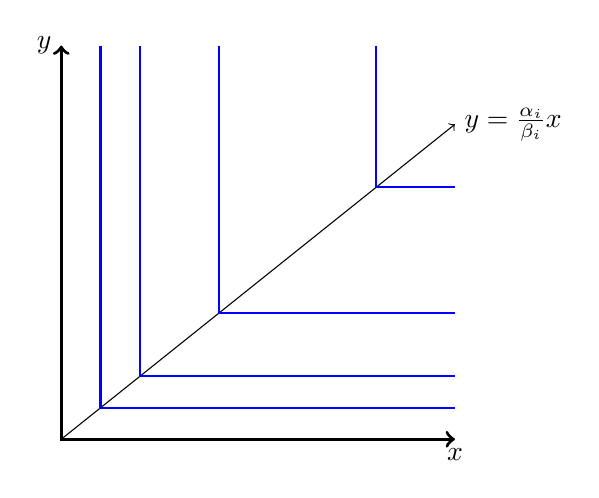
\begin{tikzpicture}[scale=0.5]
		\draw[very thick, <->] (0,10)--(0,0)--(10,0);
		\draw[->] (0,0)--(10,8);
		\node[below] at (10,0) {$x$};
		\node[left] at (0,10) {$y$};
		\draw[blue,thick] (2,10)--(2,1.6)--(10,1.6);
		\draw[blue,thick] (1,10)--(1,.8)--(10,.8);
		\draw[blue,thick] (4,10)--(4,3.2)--(10,3.2);
		\draw[blue,thick] (8,10)--(8,6.4)--(10,6.4);
		\node[right] at (10,8) {$y=\frac{\alpha_i}{\beta_i}x$};
	\end{tikzpicture}	
	\end{figure}
 	The most simple case is that in which $\frac{\alpha_1}{\beta_1} = \frac{\alpha_2}{\beta_2}$. That will look like, for \textcolor{blue}{blue} and \textcolor{red}{red} indifference curves and \textcolor{ForestGreen}{green} contract curve:
 	\begin{figure}[H]
 	\centering
 	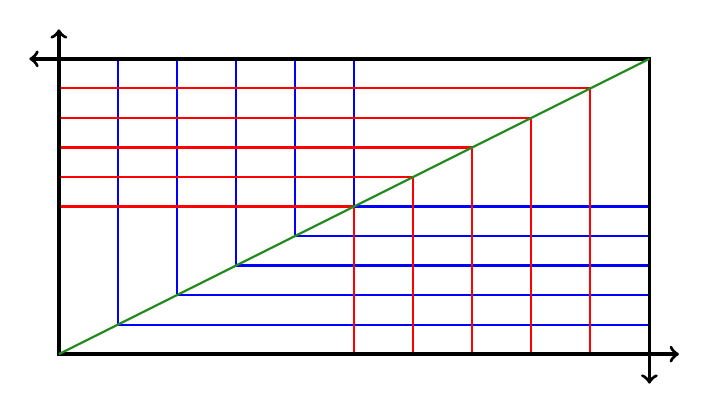
\begin{tikzpicture}[scale=0.75]
 		\draw[blue,thick] (1,5)--(1,.5)--(10,.5);
 		\draw[blue,thick] (2,5)--(2,1)--(10,1);
 		\draw[blue,thick] (3,5)--(3,1.5)--(10,1.5);
 		\draw[blue,thick] (4,5)--(4,2)--(10,2);
 		\draw[blue,thick] (5,5)--(5,2.5)--(10,2.5);
 		\draw[red,thick] (9,0)--(9,4.5)--(0,4.5);
 		\draw[red,thick] (8,0)--(8,4)--(0,4);
 		\draw[red,thick] (7,0)--(7,3.5)--(0,3.5);
 		\draw[red,thick] (6,0)--(6,3)--(0,3);
 		\draw[red,thick] (5,0)--(5,2.5)--(0,2.5);
 		\draw[very thick, <->] (0,5.5)--(0,0)--(10.5,0);
 		\draw[very thick, <->] (-0.5,5)--(10,5)--(10,-0.5);
 		\draw[thick, ForestGreen] (0,0)--(10,5);
 	\end{tikzpicture}
 	\end{figure}
 	
 	Alternatively, the slopes may not coincide. WLOG, assume that $\frac{\alpha_1}{\beta_1} < \frac{\alpha_2}{\beta_2}$, so consumer 1 requires less $y$ per $x$ than consumer 2. Note that no price vector can satisfy both consumers, as they prefer different price ratios. One good will be abundant, and its price will fall to zero. Geometrically, we have:
 	\begin{figure}[H]
 	\centering
 	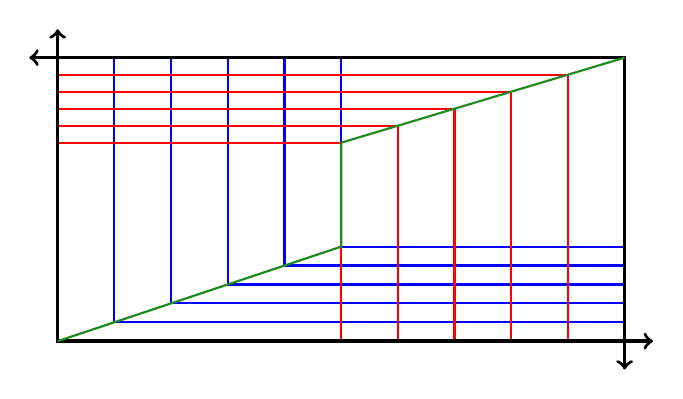
\begin{tikzpicture}[scale=0.72]
 		\draw[blue,thick] (1,5)--(1,.333)--(10,.333);
 		\draw[blue,thick] (2,5)--(2,.666)--(10,.666);
 		\draw[blue,thick] (3,5)--(3,1)--(10,1);
 		\draw[blue,thick] (4,5)--(4,1.333)--(10,1.333);
 		\draw[blue,thick] (5,5)--(5,1.666)--(10,1.666);
 		\draw[red,thick] (9,0)--(9,4.7)--(0,4.7);
 		\draw[red,thick] (8,0)--(8,4.4)--(0,4.4);
 		\draw[red,thick] (7,0)--(7,4.1)--(0,4.1);
 		\draw[red,thick] (6,0)--(6,3.8)--(0,3.8);
 		\draw[red,thick] (5,0)--(5,3.5)--(0,3.5);
 		\draw[very thick, <->] (0,5.5)--(0,0)--(10.5,0);
 		\draw[very thick, <->] (-0.5,5)--(10,5)--(10,-0.5);
 		\draw[thick, ForestGreen] (0,0)--(5,1.666)--(5,3.5);
 		\draw[thick,ForestGreen] (5,3.5)--(10,5);
 	\end{tikzpicture}
 	\end{figure}
 	\item Skipped
 	\item Skipped
 	\item Since $f$ is concave, from Jensen's Inequality we know that production is maximized by each firm taking a share $L / n$ of the total labor endowment, so the aggregate production possibility set is described by $n f(L / n)$. Note that this is equivalent to \[L \cdot \frac{f(L/n)}{L/n}\]As $n$ increases, the limit becomes:\[\lim_{n\to\infty} L \cdot \frac{f(L/n)}{L/n} = L \lim_{x \to 0} \frac{f(x)}{x} = L \cdot f'(0) = L\cdot b\]Thus, the PPS converges to as if we had linear technology as $n$ increases, because each firm is using closer and closer to 0 labor. Note that this actually increases the marginal product of each worker, and thus the aggregate product, since $f$ is concave. \\\\ Note that if $f(x) = \sqrt{x}$, we now have that $f'(0) \to  \infty$. Thus, the marginal product of each worker increases infinitely as $n$ increases, so the PPS grows to encompass the entire positive orthant, as the marginal product of each worker at 0 is infinite.
\end{enumerate}






















\end{document}